
            \begin{figure}[h]
                \centering
                \begin{tikzpicture}
                    %图片
                    \node  at (0,0) {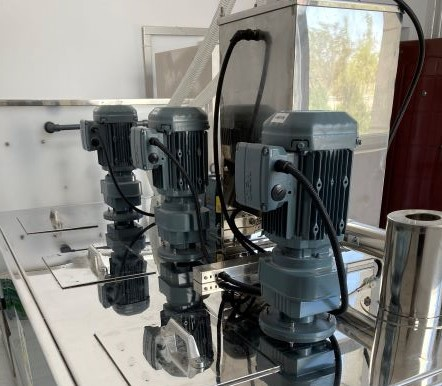
\includegraphics[height=5.5cm]{g15.JPG}};

                    %说明
                    \node at (-5,2) (2) [text_box] {料斗高料位探头};
                    \draw [arrow] (2) -- (0.5,2.2);
                    \draw (0.5,2.2) circle (0.5)[red];
                    \node at (-5,-1) (1) [text_box] {料斗低料位探头};
                    \draw [arrow] (1) -- (0.5,-0.2);
                    \draw (0.5,-0.2) circle (0.5)[red];

                    %辅助线
                    % \draw (-8,-2) [help lines] grid (8,2);
                    % \draw [red] (-8,0) -- (8,0);
                    % \draw [red] (0,-2) -- (0,2);
                \end{tikzpicture}
                \caption{料斗高低料位探头}\label{fig:p12}
            \end{figure}
